
\section{Simple boundary conditions}

Any fluid flow model cannot be build without including of the influence of the surrounding environment. This influence can be described mathematically with so called boundary conditions. If the boundary conditions are not set, then at the end all the probability densities will be streamed out of the domain with the streaming step. Boundary conditions build the external constraints which influence the solution of the whole system. The implementation of the boundary conditions in LBM is straightforward, but the mathematical background of these boundary conditions may be even more complicated than the LBM itself.

One of the easiest boundary conditions is a no-slip (see Fig. \ref{fig:no-slip-BC}). The no-slip boundary conditions are used in case of real walls or obstacles, which offer a certain amount to friction of the fluid. In the case when the fluid velocity at the wall is reduced to zero, the boundary conditions can be implemented in the following way: all distribution functions of a fluid cell neighboring an obstacle cell pointing towards the obstacle are simply reversed \cite{pflaum}. This assures that the fluid velocity normal and tangential to the wall are zero. These are so called Dirichlet boundary conditions.

\begin{figure}[H]
  \centering
  \begin{subfigure}[h]{0.3\textwidth}
    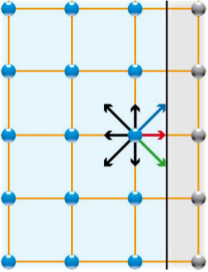
\includegraphics[width=\textwidth]{img/fig8-1.png}
  \end{subfigure}
  \begin{subfigure}[h]{0.3\textwidth}
    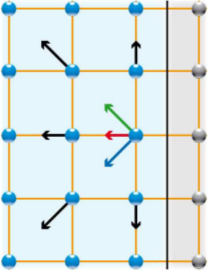
\includegraphics[width=\textwidth]{img/fig8-2.png}
  \end{subfigure}
  \caption{No-slip boundary conditions. Left - before streaming step; Right – after streaming step \cite{pflaum}.}\label{fig:no-slip-BC}
\end{figure}

The next simple boundary conditions are free-slip boundary conditions (see Fig. \ref{fig:free-slip-BC}). They can be used if there are walls without friction. A usual example of free-slip boundary conditions is at symmetry axes in certain simulation domains, for example in the middle of a channel flow. The free-slip boundary conditions are applied as follows: all distribution functions of a fluid cell neighboring a free-slip boundary pointing towards the boundary are reflected in their component normal to the wall. This assures that the velocity normal to the wall is zero, whereas the velocity tangential to the wall remains unchanged \cite{pflaum}. These are so called Neumann boundary conditions:

\begin{equation}
\frac{\partial v_t}{\partial n} = 0.
\end{equation}

\begin{figure}[H]
  \centering
  \begin{subfigure}[h]{0.3\textwidth}
    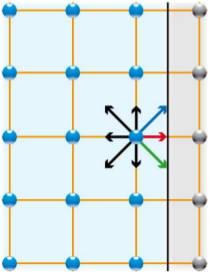
\includegraphics[width=\textwidth]{img/fig9-1.png}
  \end{subfigure}
  \begin{subfigure}[h]{0.3\textwidth}
    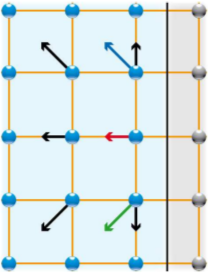
\includegraphics[width=\textwidth]{img/fig9-2.png}
  \end{subfigure}
  \caption{Free-slip boundary conditions. Left - before streaming step; Right – after streaming step \cite{pflaum}.}\label{fig:free-slip-BC}
\end{figure}

To implement the lid-driven cavity, which will be described in the next section, more boundary conditions are needed. Such boundary conditions are called bounce-back condition with additional acceleration (see Eq. 21) and used to model a moving wall. Such boundaries are used to implement a wall that moves with some certain velocity, which is imparted to the fluid particles, accelerating the fluid. These boundaries are similar to no-slip boundaries except for the scaling term depending on the wall velocity \cite{pflaum}:

\begin{equation}
f_{\bar{\alpha}}(\vec{x},t) = f_{\alpha}(\vec{x},t) - 2 t_p \rho \frac{3}{c^2} c_{\alpha} u_{w}
\end{equation}
where $\alpha$ is the direction towards the wall, $\bar{\alpha}$ is the reverse direction from the wall, $t_p$ is the direction dependent parameter, $\rho$ is the fluid density of the near wall fluid cell, and $u_w$ is the wall velocity.
